\documentclass{article}
\usepackage{listings}
\usepackage{setspace}
\usepackage{geometry}
\usepackage{graphicx}
\usepackage{float}
\usepackage[spanish]{babel}

\geometry{a4paper, top=1in, bottom=1in, left=1in, right=1in}
\doublespacing


\begin{document}

\title{
\includegraphics[width=0.3\textwidth]{imagenes/logo_ufro.png}\\[0.1cm]Números adyacentes}
\author{Matías Hoyuela, Eduardo Vásquez, Francisco Cáceres}
\date{\today}
\maketitle

\section{Introducción}
El informe presenta los pasos realizados para resolver el problema de buscar el mayor producto de números adyacentes en un arreglo.

\section{Descripción del caso}
Dado el arreglo:
\begin{lstlisting}[language=Java]
    new double[]{1, -4, 2, 2, 5, -1}
\end{lstlisting}
Se debe de implementar un método que retorne el mayor producto de números adyacentes. En este caso, el mayor producto es 10, con los números 2 y 5.

\section{Análisis del caso}

Se planifica el método:

\begin{itemize}
    \item Parámetros de entrada: un arreglo de números \texttt{double[]}.
    \item Valor de retorno: el mayor producto de números adyacentes \texttt{double}.
    \item Instrucciones: iterar sobre el arreglo de entrada e ir actualizando una variable cada vez que se encuentre un producto entre 2 números adyacentes mayor al valor de la variable, retornar el valor de la variable e imprimir en la consola el resultado.
\end{itemize}

\section{Implementación de la solución}

\begin{figure}[H]
    \centering
    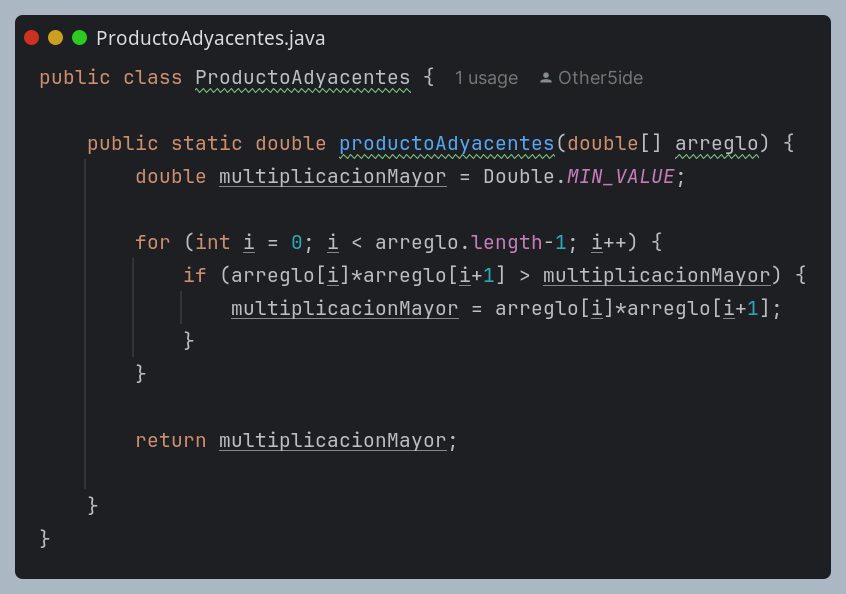
\includegraphics[width=0.8\textwidth]{imagenes/solutionv1.png}
\end{figure}

Para la solución, se inicializa una variable \texttt{double multiplicacionMayor}, y luego se itera sobre el arreglo. En cada iteración, se compara el producto de \texttt{arreglo[i]} y \texttt{arreglo[i+1]} con la variable \texttt{multiplicacionMayor}, y si el producto es mayor a esta, se actualiza la variable con ese producto.
Para evitar un error de \texttt{ArrayIndexOutOfBoundsException}, se itera hasta \texttt{arreglo.length - 1}, por que si fuera hasta \texttt{arreglo.length}, durante la iteración \texttt{i = arreglo.length}, \texttt{arreglo[i+1]} intentaría acceder a un índice que no existe y lanzaría la excepción. Una vez se termina la iteración, se retorna else valor final de \texttt{multiplicacionMayor}.

\section{Diseño-implementación de las pruebas unitarias}

Se pensaron las siguientes pruebas:
\begin{itemize}
    \item Arreglo de un solo elemento. El método debe lanzar una excepción IllegalArgumentException, puesto que se requiere un arreglo de al menos 2 elementos para calcular el producto de números adyacentes.
    \item Un arreglo vacío. Nuevamente, el método debe lanzar IllegalArgumentException, puesto que se requiere un arreglo de al menos 2 elementos.
    \item Arreglo nulo. El método debe lanzar una excepción IllegalArgumentException, puesto que el arreglo no puede ser nulo.
    \item Arreglo negativo. El método debe retornar el mayor producto de números adyacentes, considerando los signos durante la multiplicación y la comparación.
    \item Arreglo con un NaN. El método debe lanzar IllegalArgumentException, puesto que NaN no es valido para la multiplicación.
    \item Arreglo con un infinito. El método debe lanzar IllegalArgumentException, puesto que infinito no es valido para la multiplicación.
    \item Arreglo con un producto infinito. El método debe lanzar ArithmeticException, puesto que el producto debe ser finito.
\end{itemize}
Esto considerando que el input cumple con las siguientes condiciones:
\begin{itemize}
    \item \texttt{2 <= arreglo.length <= 1000}
    \item \texttt{-1000 <= arreglo[i] <= 1000}
\end{itemize}
Tras diseñar las pruebas en papel, se implementaron en el programa:
\begin{figure}[H]
    \centering
    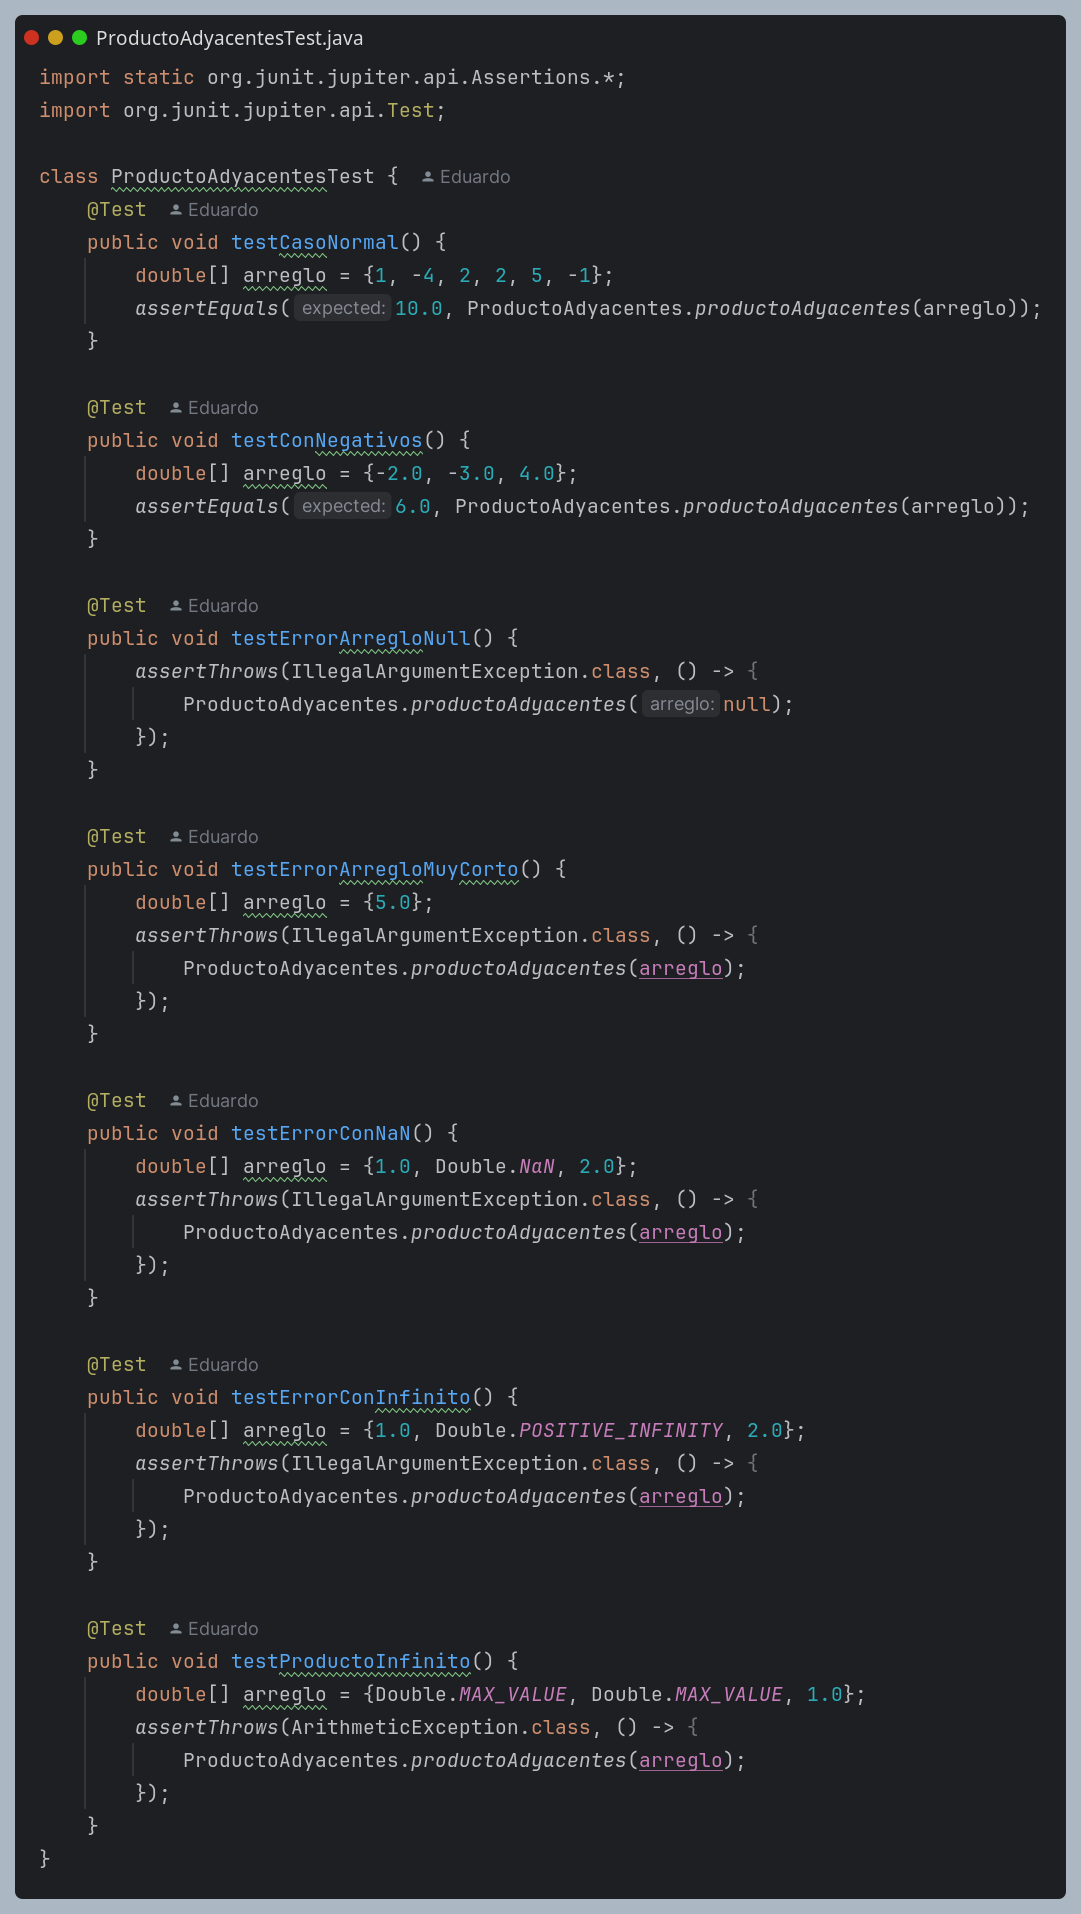
\includegraphics[width=0.8\textwidth]{imagenes/unittest.png}
\end{figure}
Resumen de las pruebas:
\begin{itemize}
    \item \texttt{testCasoNormal}: prueba con el arreglo de ejemplo del ejercicio.
    
    \begin{itemize}
        \item Entrada: \texttt{double arreglo[] = \{1, -4, 2, 2, 5, -1\}}
        \item Salida: \texttt{10}
    \end{itemize}

    \item \texttt{testConNegativos}: prueba con un arreglo que contiene números negativos.

    \begin{itemize}
        \item Entrada: \texttt{\{-2.0, -3.0, 4.0\}}
        \item Salida: \texttt{6.0}
    \end{itemize}

    \item \texttt{testErrorArregloNulo}: prueba con un null.
    
    \begin{itemize}
        \item Entrada: \texttt{null}
        \item Salida: \mbox{\texttt{IllegalArgumentException}}
    \end{itemize}

    \item \texttt{testErrorArregloMuyCorto}: prueba con un arreglo de solo un elemento.
    
    \begin{itemize}
        \item Entrada: \texttt{double arreglo[] = \{5.0\}}
        \item Salida: \texttt{IllegalArgumentException}
    \end{itemize}

    \item \texttt{testErrorConNan}: prueba con un arreglo que contiene un NaN.
    
    \begin{itemize}
        \item Entrada: \texttt{double arreglo[] = \{1.0, Double.NaN, 2.0\}}
        \item Salida: \texttt{IllegalArgumentException}
    \end{itemize}

    \item \texttt{testErrorConInfinito}: prueba con un arreglo que contiene un infinito.
    
    \begin{itemize}
        \item Entrada: \texttt{double[] arreglo = \{1.0, Double.POSITIVE\_INFINITY, 2.0\}}
        \item Salida: \texttt{IllegalArgumentException}
    \end{itemize}

    \item \texttt{testProductoInfinito}: prueba con un arreglo que el mayor producto de números adyacentes es infinito.
    
    \begin{itemize}
        \item Entrada: \texttt{double[] arreglo = \{Double.MAX\_VALUE, Double.MAX\_VALUE, 1.0\}}
        \item Salida: \texttt{ArithmeticException}
    \end{itemize}

\end{itemize}


\section{Diseño-implementación y resultados de las excepciones implementadas}
Se modificó el programa para que gestione las excepciones y pase las pruebas:
\begin{figure}[H]
    \centering
    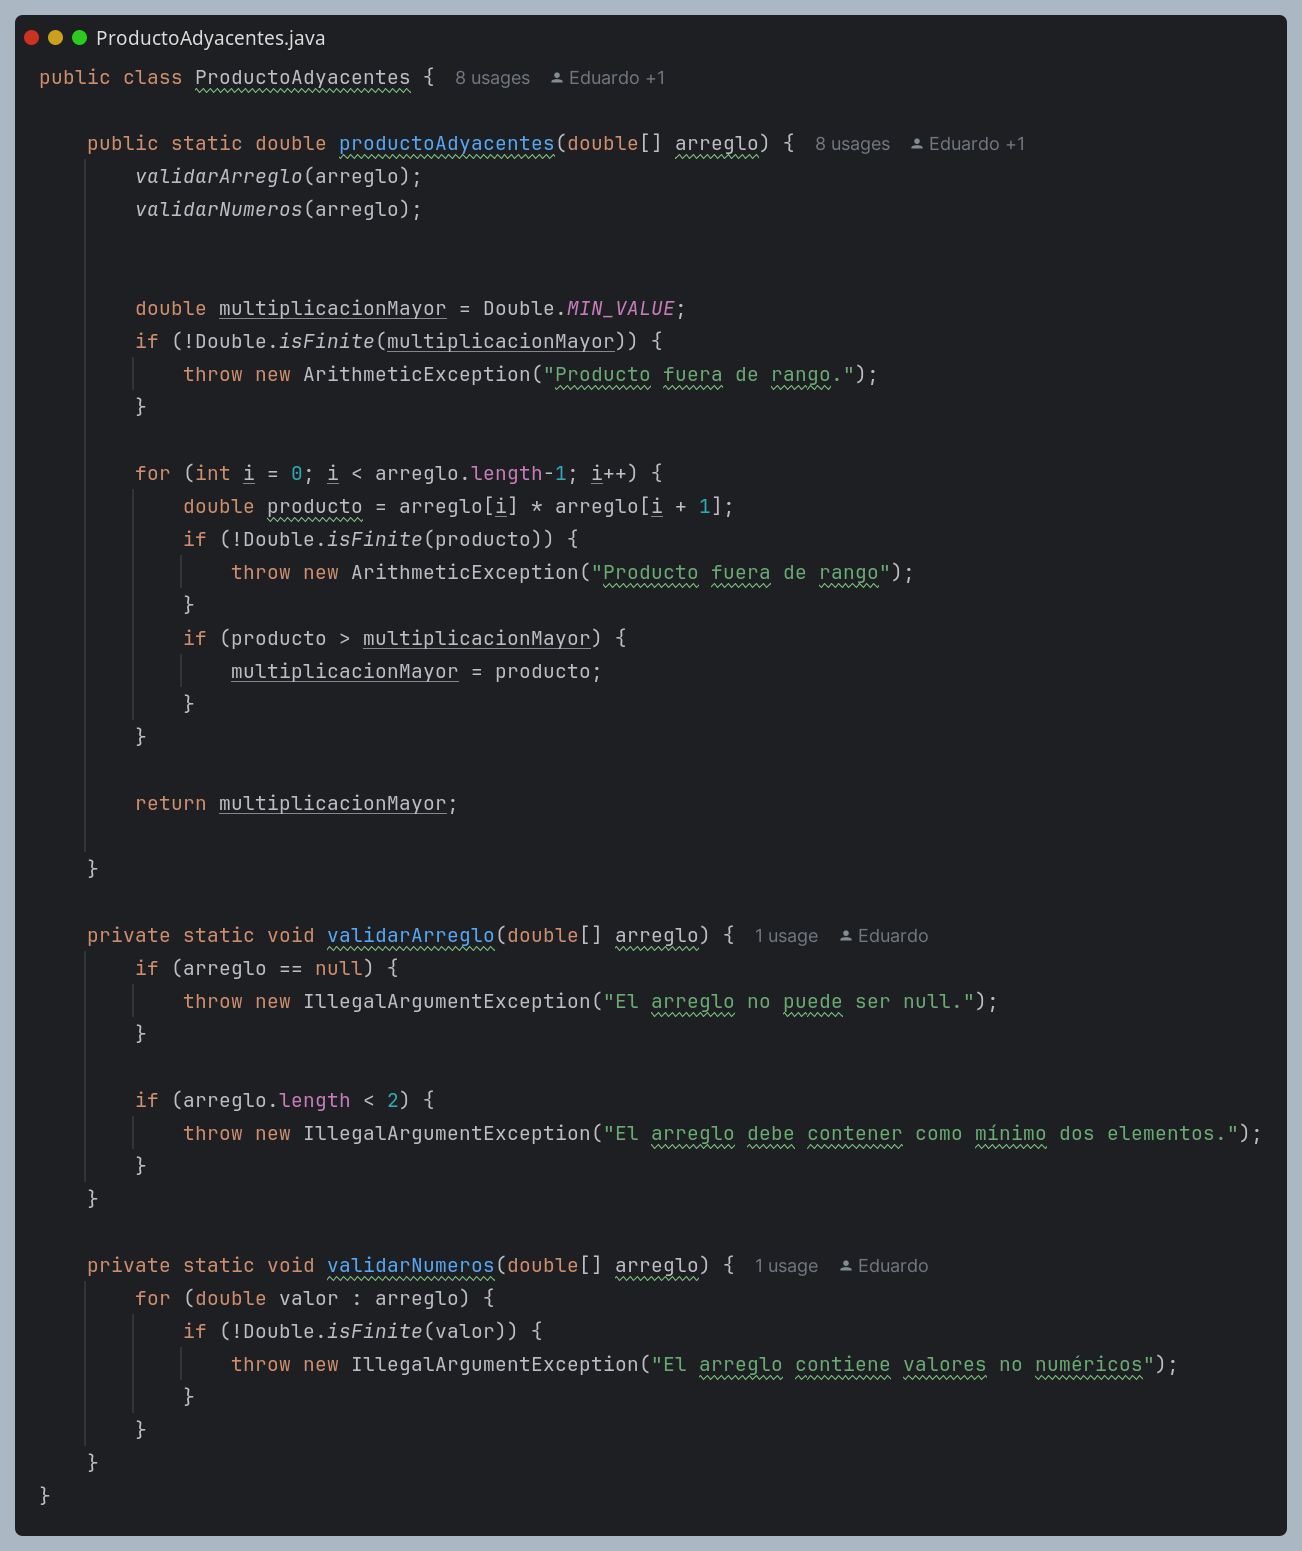
\includegraphics[width=0.8\textwidth]{imagenes/solutionv2.png}
\end{figure}
\begin{itemize}
    \item Primero, el método \texttt{validarArreglo} verifica que el arrelgo no sea null y que contenga al menos 2 elementos. Si no cumple con ninguna de estas condiciones, lanza una IllegalArgumentException.
    \item Luego, el método \texttt{validarNumeros} itera sobre el arreglo para verificar que no contenga valores no numéricos. Si encuentra alguno, lanza una IllegalArgumentException.
    \item Por último, durante la busqueda del producto mayor, si alguno de los productos es infinito, se lanza una ArithmeticException.
\end{itemize}


\section{Discusión con los resultados y comentarios de la experiencia}

\section{Conclusiones}

Gracias a las pruebas unitarias, se pudo hacer un programa más robusto, que en un inicio, requería que el usuario ingresara un arreglo que cumpla con ciertas reglas. Sin embargo, como aprendimos en clases, no se puede confiar en el usuario, por tanto, el programa debe de ser capaz de manejar todo tipo de entradas, y no solo las que cumplen con las reglas. Para esto, se implementaron las excepciones, que hacen que el programa, pueda identificar y manejar entradas no válidas, como arreglos de un solo elemento, que contengan elementos no válidos, etc. De esta forma, el programa funciona en cualquier caso, y no depende de que el usuario siga nuestras reglas.

\end{document}